% % % % % % % % % % % % % % % % % % % % % % % % % % % % % % % % % % % % % % % %
% LaTeX4EI Template for Cheat Sheets                                Version 1.1
%
% Authors: Markus Hofbauer
% Contact: info@latex4ei.de
% Encode: UTF-8
% % % % % % % % % % % % % % % % % % % % % % % % % % % % % % % % % % % % % % % %


% ======================================================================
% Document Settings
% ======================================================================

% possible options: color/nocolor, english/ngerman, threecolumn
% defaults: color, english
\documentclass[ngerman, threecolumn, 8pt]{latex4ei/latex4ei_sheet}

% set document information
\title{Computertechnik}
\author{Darius Peters}                    % optional, delete if unchanged
\myemail{darius.peters@tum.de}           % optional, delete if unchanged
\mywebsite{www.latex4ei.de}          % optional, delete if unchanged


%Packages
\usepackage{pdfpages}
\usepackage{xcolor}
\usepackage{fancyhdr}
\usepackage{lastpage}

%Custom Commands
\newcommand{\imglog}{\includegraphics[width=.70cm]}

%custom settings
\titlespacing*{\subsection}{.5pt}{.5pt}{2pt}
\titlespacing*{\subsubsection}{0pt}{.5pt}{2pt}


% ======================================================================
% Begin
% ======================================================================
\begin{document}

\lfoot{Nur zur persöhnlichen Verwendung!}

\IfFileExists{git.id}{\input{git.id}}{}
\ifdefined\GitRevision\mydate{\GitNiceDate\ (git \GitRevision)}\fi

% Title
% ----------------------------------------------------------------------
\maketitle   % requires ./img/Logo.pdf
\\
\textcolor{red}{\small Diese Formelsammlung ist für den privaten Gebrauch und das Selbststudium von Studierenden erstellt worden. Die Inhalte basieren auf Materialien des Lehrstuhls für Datenverarbeitung und sind ausschließlich zur Unterstützung des Lernens gedacht.}
% Section
% ----------------------------------------------------------------------
\section{Zahlen und Zeichen}
    \subsection{Daten als Bits und Bytes}
	\subsubsection{Binärdarstellung}
	1 - High Pegel - logisch wahr\\
	0 - Low Pegel - logisch falsch
	\subsubsection{Hexadezimaldarstellung}
	Zusammenfassen von 4 Bits zu 0, 1, ..., E,D F\\
	\begin{tabular}{l|l||l|l}
	0: 0000 & 1: 0001 & 8: 1000 & 9: 1001\\
	2: 0010 & 3: 0021 & A: 1010 & B: 1011\\
	4: 0100 & 5: 0101 & C: 1100 & D: 1101\\
	6: 0110 & 7: 0111 & E: 1110 & F: 1111\\
	\end{tabular}
	\subsubsection{Bits/Bytes (MMIX)}
	\begin{itemize}\itemsep0pt
	\item1 Byte = 8 Bits = 1 Byte
	\item2 Byte = 16 Bits = 1 Wyde
	\item4 Byte = 32 Bits = 1 Tetra
	\item8 Byte = 64 Bits = 1 Octa
	\end{itemize}
	\begin{sectionbox}
	\subsubsection{ASCII-Tabelle}
	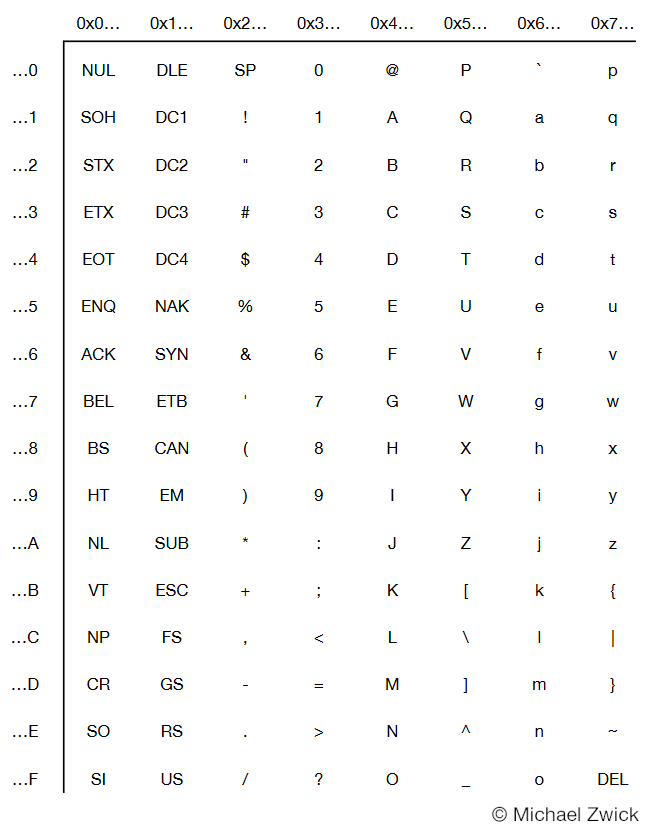
\includegraphics[width=.85\linewidth]{./img/ascii_table.png}
	\end{sectionbox}
	\subsection{Zahlen}
	\subsubsection{Vorzeichenlose Festkommazahlen}
	\textbf{Definition:} $v=(a_{n-1} \cdot b^{n-1}+\dots+a_1 \cdot b^1 + a_0 \cdot b^0) \cdot b^r$\\
	$b$: Basis (meist 2); $n$: Stellenzahl; $a \in 0 \dots (b-1)$; $r$: Position des Kommas
	\subsubsection{Einer Komplement}
	Vorzeichen wird durch MSB abgelesen\\
	Umwandlung durch invertieren aller Bits
	\subsubsection{Zweier Komplement}
	Vorzeichen wird durch MSB abgelesen\\
	Umwandlung durch invertieren aller Bits und binärer Addition des Werts 1 (von positiv zu negativ)


	\subsubsection{Gleitkommazahlen nach IEEE 754}
	Bestehend aus: Vorzeichen ($s$), Exponentteil ($e$), Mantisse ($f$)\\
	Vorgehen (Bsp. $17,625$): 
	\begin{enumerate}
	\item Zahl vor dem Komma ($17,0$) und nach dem Komma ($0,625$) getrennt in binär umwandeln
	\item Zusammen in binär schreiben ($10001,101$)
	\item Das Komma durch Anpassung des Exponenten $e-K$, verschieben, um das Format $1,f$ zu erhalten ($1,0001101 \cdot 2^4 \rightarrow e-K=4$) \\
	\end{enumerate}
\begin{sectionbox}
	Definition (normalisiert): $v=(-1)^s \cdot 1,f \cdot 2^{e-K}$\\\\
    \textbf{32 Bit:}
        \begin{itemize}\itemsep0pt
            \item $K=127$
            \item $s = 1$ Bit
            \item $e = 8$ Bit
            \item $f = 23$ Bit
        \end{itemize}
    \textbf{64 Bit:}
        \begin{itemize}\itemsep0pt
            \item $K=1023$
            \item $s = 1$ Bit
            \item $e = 11$ Bit
            \item $f = 52$ Bit
        \end{itemize}
	\textbf{Spezialfälle} (de-normalisiert):
	\begin{itemize}\itemsep0pt
	\item 0: $e=0$; $f=0$
	\item $+\infty$: $e=1\dots1$; $f=0$; $s=0$
	\item $-\infty$: $e=1\dots1$; $f=0$; $s=1$
	\item \text{Not a Number}: $e=1\dots1$; $f>0$
	\end{itemize}
\end{sectionbox}

\section{Arithmetische Schaltungen}
\begin{sectionbox}
\subsection{Schaltungselemente}
\begin{tabular}{c|c!{\vrule width 0.75pt}c|c|c|c|c|c}
		& & \imglog{img/logic/not-us.png} & \imglog{img/logic/and-us.png} & \imglog{img/logic/or-us.png} & \imglog{img/logic/xor-us.png} & \imglog{img/logic/nand-us.png} & \imglog{img/logic/nor-us.png}\\
		x & y &    Inverter     &    AND     &  OR   &     XOR     &         NAND          &       NOR        \\
		  &   & $\overline{x}$ & $x\wedge y$ & $x\vee y$ & $x\oplus y$ & $\overline{x\wedge y}$ & $\overline{x\vee y}$ \\ \hline\hline
		0 & 0 &     1      &     0      &   0   &      0      &           1           &        1         \\ \hline
		0 & 1 &     1      &     0      &   1   &      1      &           1           &        0         \\ \hline
		1 & 0 &     0      &     0      &   1   &      1      &           1           &        0         \\ \hline
		1 & 1 &     0      &     1      &   1   &      0      &           0           &        0         
	\end{tabular}\\ \\
	Ein \textit{Treiber} besteht aus zwei Invertern in Serie geschalten.
\end{sectionbox}
\subsection{Fan-In/Fan-Out}
Fan-In: max. Eingänge in Gatter \\
Fan-Out: max. Ausgänge aus Gatter
\subsection{Multiplexer}
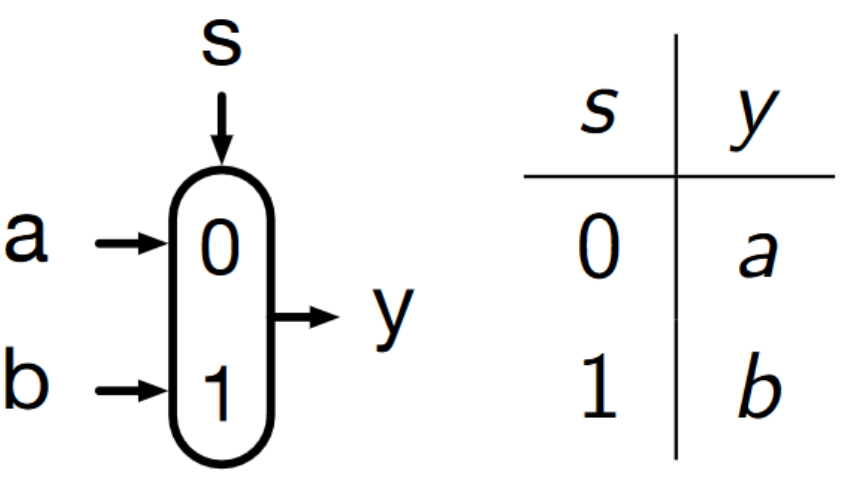
\includegraphics[width=2cm]{img/logic/multiplexer.png}
\subsection{Ripple-Carry-Addierer}
Berechnung der Summe aus zwei Summanden \\
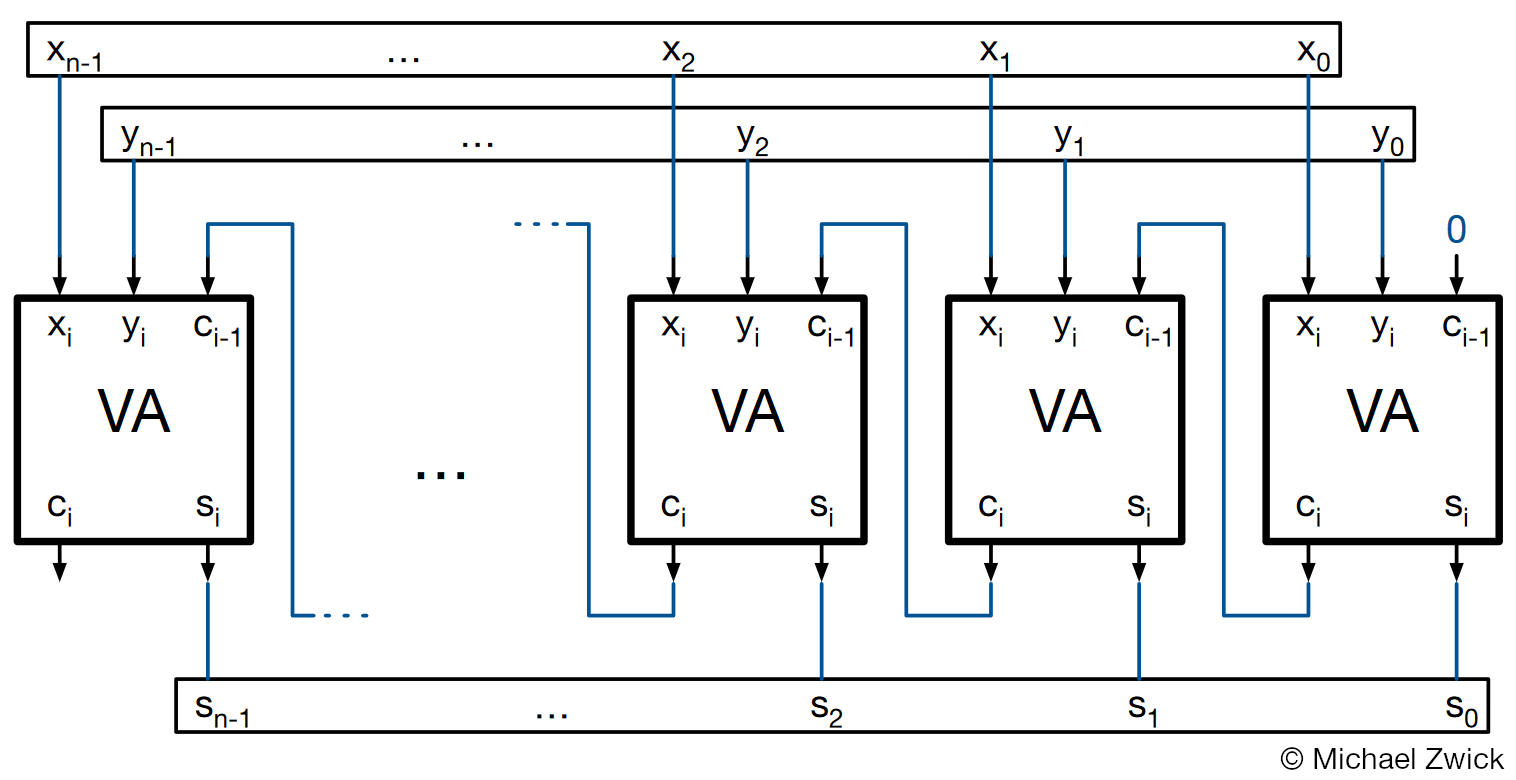
\includegraphics[width=.9\linewidth]{img/rca/rca.png} \\
\subsection{Carry-Look-Ahead}
Schnellere Berechnung der Summe aus zwei Summanden durch zusätzliche Logik zur Bestimmung des Übertrags\\
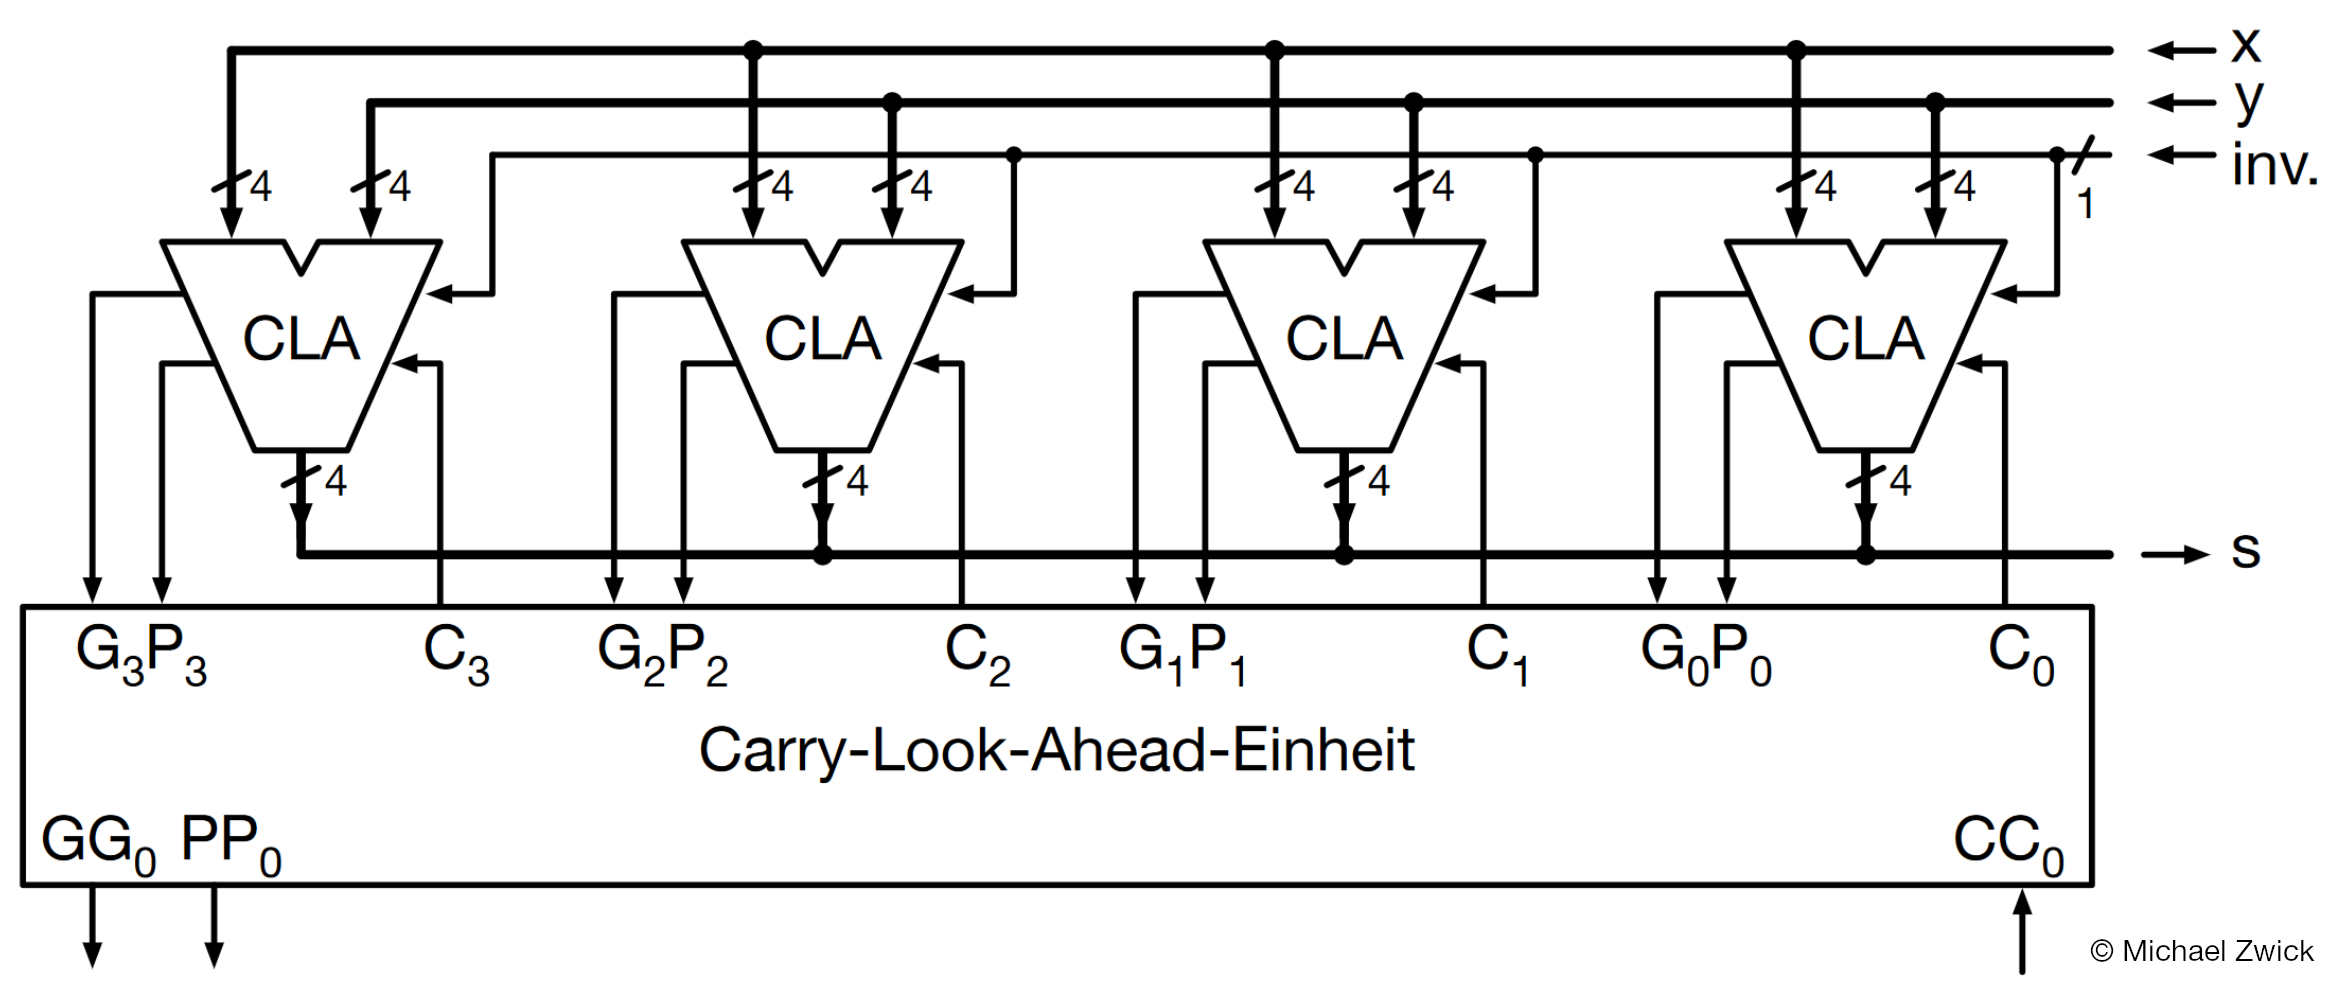
\includegraphics[width=.95\linewidth]{img/rca/cla.png} \\
Überlauf ($c_i$) eines Volladdierers:\\
$c_i=g_i \lor (p_i \land g_{i-1}) \lor (p_i \land p_{i-1} \land g_{i-2}) \lor \dots$\\
\subsection{Zustandsautomat}
\begin{center}
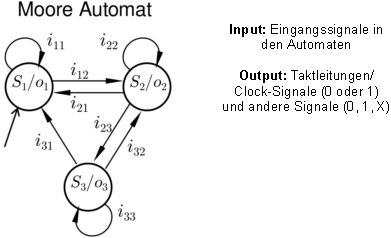
\includegraphics[width=.8\linewidth]{img/moore-automat.pdf}
\end{center}
%\begin{itemize}
%\item Input: Eingangssignale in den Automaten
%\item Output: Taktleitungen/Clock-Signale (0 oder 1) und andere Signale (0, 1, X)
%\end{itemize}
\begin{sectionbox}
\subsection{ROM-Steuerung}
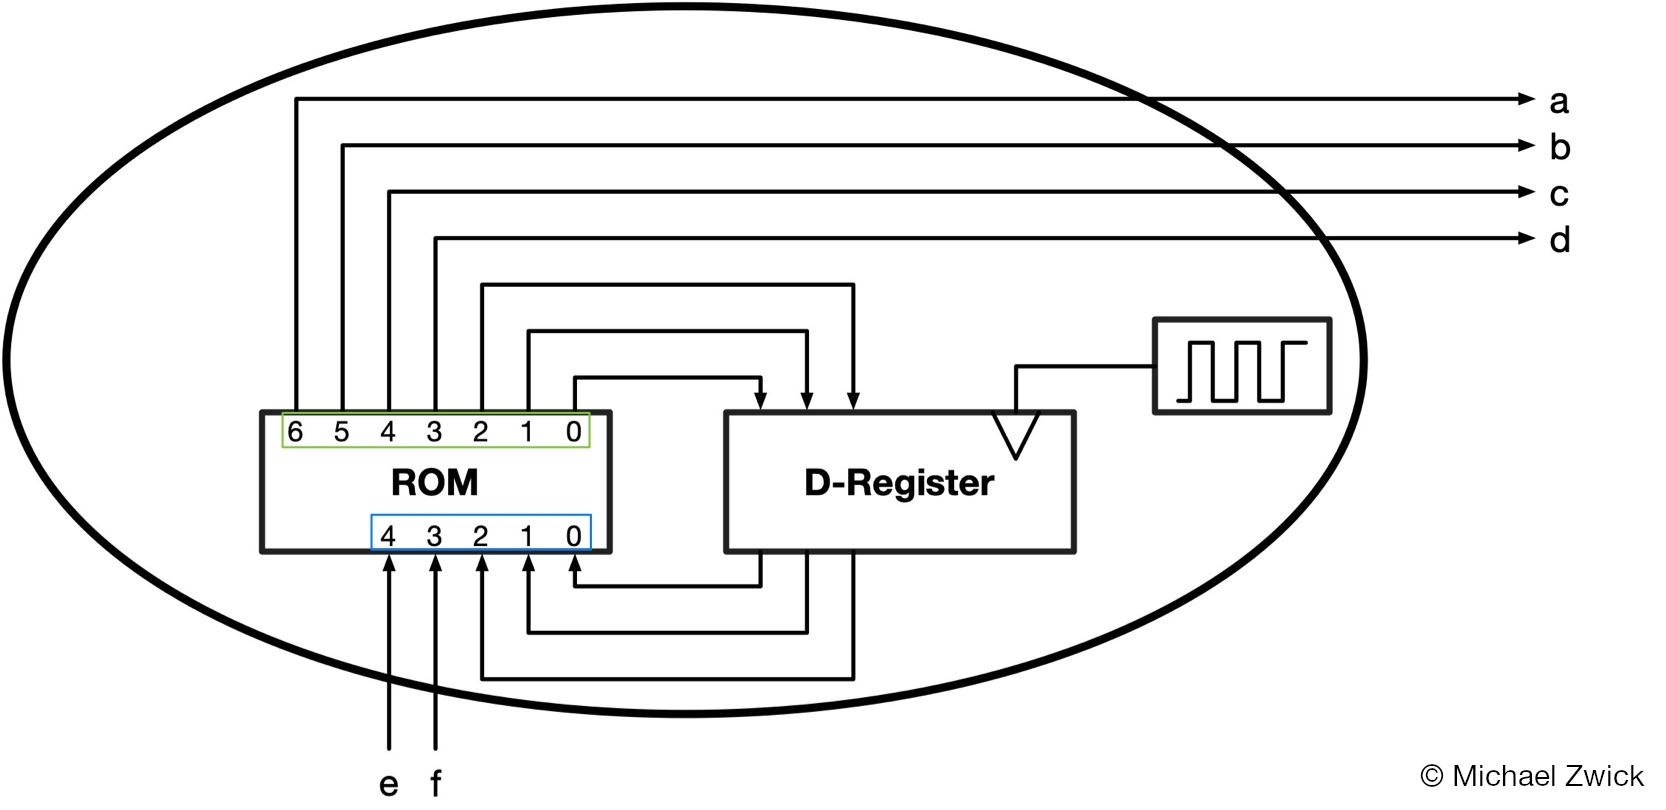
\includegraphics[width=.85\linewidth]{img/ROM-Steuerung.jpg} \\
Tabelle mit \textcolor{blue}{Eingabe} (gegeben) und \textcolor{green}{Ausgabe} (auszufüllen) \\
Vorgehen: Einträge der gegebenen Tabelle in Binärzahlen umwandeln. Bits $0, 1, 2$ der Eingabe sind der derzeitige Zustand. Bits $3, 4, \dots$ der Eingabe sind die Eingangssignale für den nächsten Zustand. Bits $0, 1, 2$ der Ausgabe sind der Folgezustand und Bits $3, 4, \dots$ die Ausgangssignale des aktuellen Zustands.\\
\textbf{Ansatz:} \\
\begin{tabular}{c c|c c}
e f & Zst. & a b c d & Folgezst.\\
(4 3) & (2 1 0) & (6 5 4 3) & (2 1 0) \\ \hline
\textcolor{blue}{\dots} &  \textcolor{blue}{\dots} & \textcolor{green}{\dots} & \textcolor{green}{\dots} \\
 \textcolor{blue}{\dots} &  \textcolor{blue}{\dots} & \textcolor{green}{\dots} & \textcolor{green}{\dots} \\
\end{tabular}
\end{sectionbox}
\begin{sectionbox}
\subsection{Universalrechner}
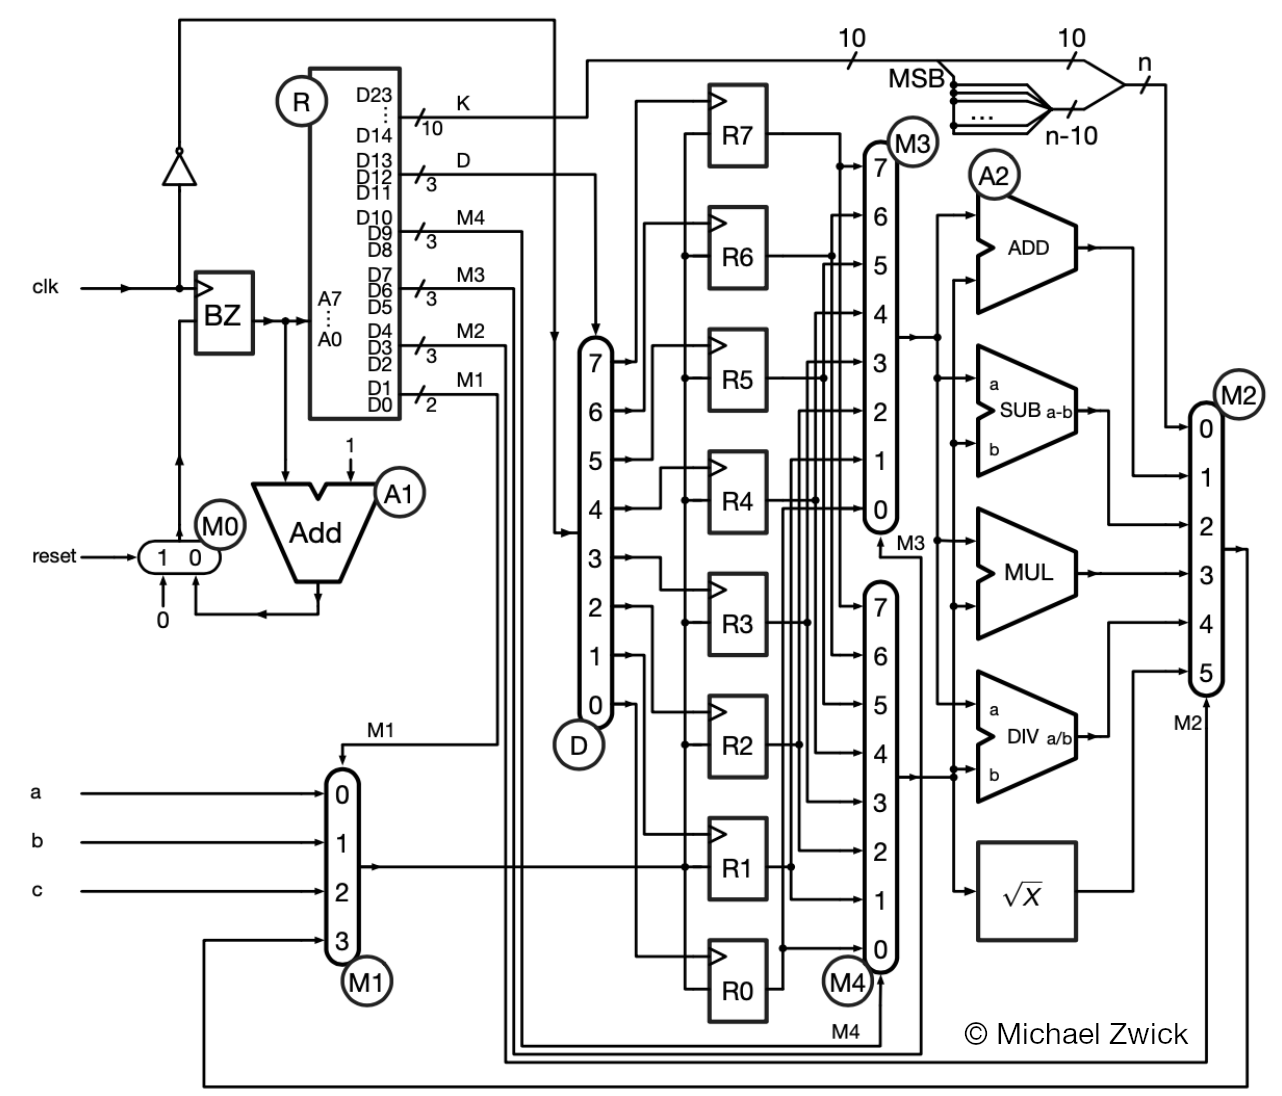
\includegraphics[width=.9\linewidth]{img/Universalrechner.png} \\
\textbf{Auch hier gilt:} Klammer \textit{vor} Potenz \& Wurzel \textit{vor} Punkt \textit{vor} Strich!
\begin{itemize}\itemsep0pt
\item \textbf{K:} Konstante
\item \textbf{D:} Ziel-Register
\item \textbf{M1:} Ergebnis-Auswahl
\item \textbf{M2:} Rechenoperation/Konstante-Laden
\item \textbf{M3:} Operand 1 \textit{(bei $\sqrt{x}$ jedoch M4 verwenden)}
\item \textbf{M4:} Operand 2
\end{itemize}
\end{sectionbox}
\begin{minipage}{\columnwidth}
\section{MMIX-Architektur}
\subsection{Big-Endian und Little-Endian}
\textbf{Big-Endian:} höherwertigeres Byte wird adressiert (von links nach rechts)\\
\textbf{Little-Endian:} niederwertigeres Byte wird adressiert (von rechts nach links)\\
\begin{sectionbox}
\subsection{Übersetzungstabelle}
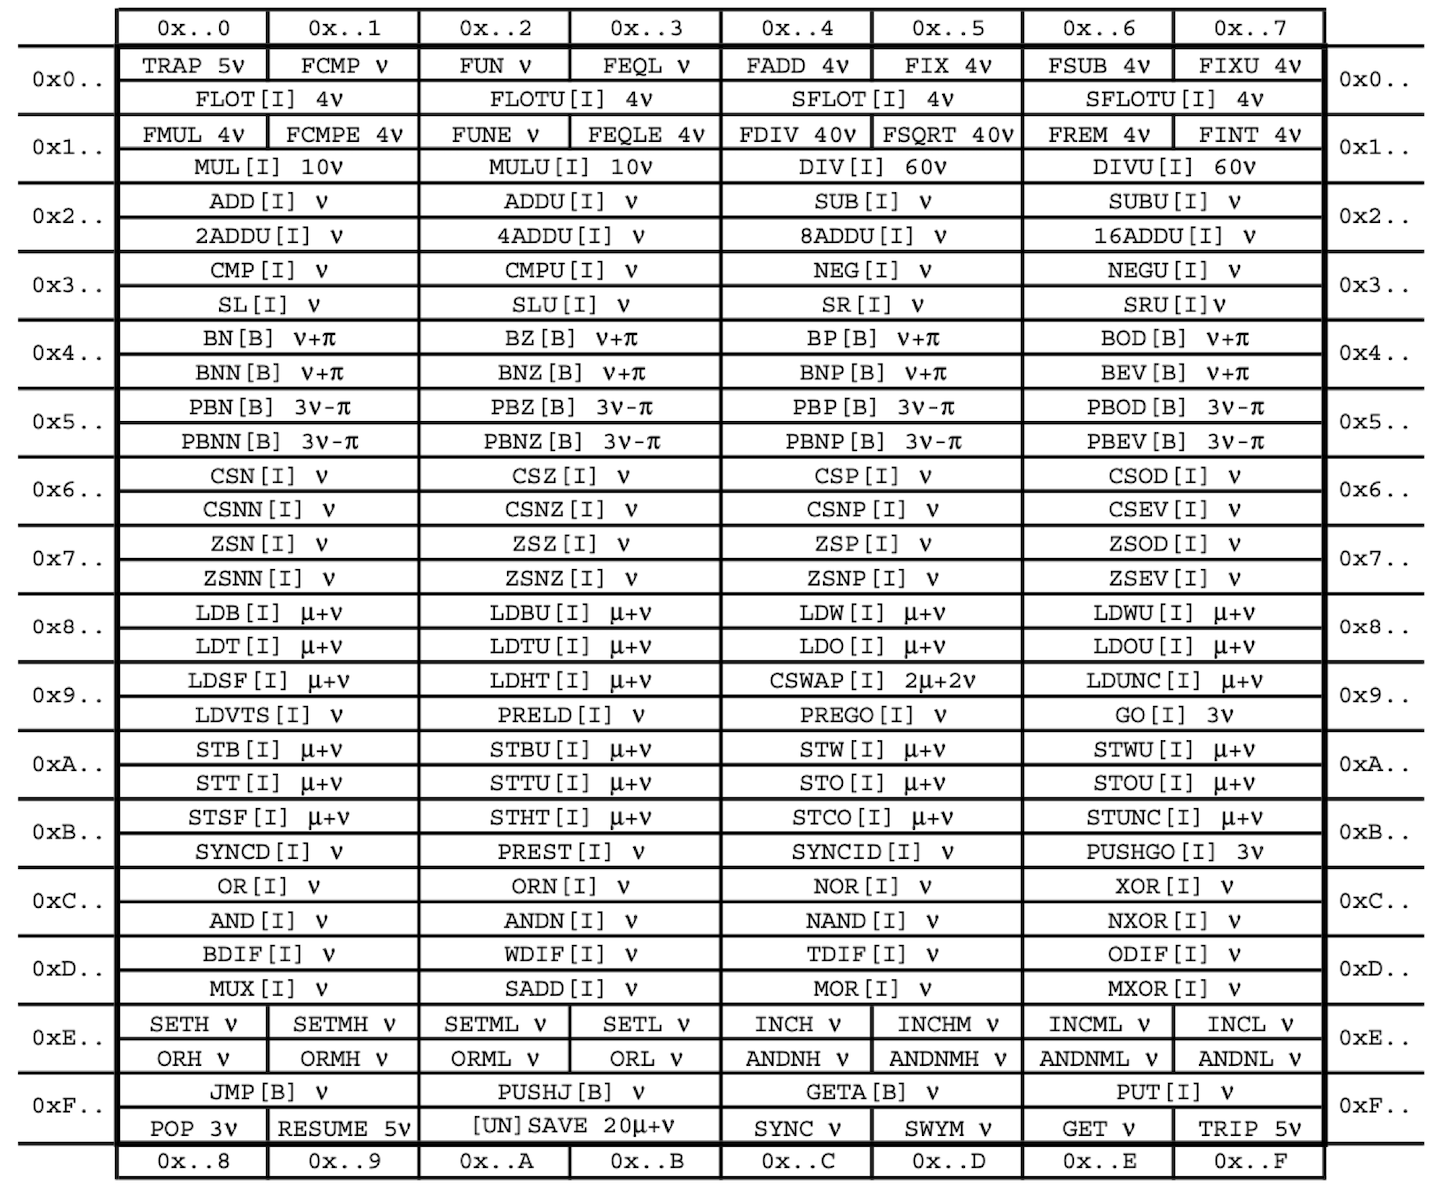
\includegraphics[width=\linewidth]{img/Uebersetzungstabelle.png}
Um Opcode zu erhalten erste Hex-Zahl links ablesen, zweite Hex-Zahl oben/unten ablesen (je nachdem ob Befehl in oberer oder unterer Zeile)\\
$I$: immideate (Direktoperand); $B$: backwards (bei Sprungbefehlen)
\end{sectionbox}
\end{minipage}
\subsection{Spezielle Befehle}
\subsubsection{Namensraum}
Namensraum eröffnen: \texttt{PREFIX Name} \\
Namensraum beenden: \texttt{PREFIX :}
\subsubsection{Stack-Pointer (SP)}
\begin{itemize}
\item n Register auf Stack ablegen: \\
1. SP anpassen: \texttt{SUB, :SP, :SP, 8*n}\\
2. Mit \texttt{STO} speichern
\item n OCTAs aus Stack einlesen: \\
1. Mit \texttt{LDO} einlesen\\
2. SP anpassen: \texttt{ADD, :SP, :SP, 8*n}
\end{itemize}
\subsection{Alignment}
\subsubsection{In den Speicher}
\begin{itemize}\itemsep0pt
\item \textbf{BYTE:} geht immer
\item \textbf{WYDE:} letztes Bit muss 0 sein 
\item \textbf{TETRA:} letzten beiden Bits müssen 0 sein 
\item \textbf{OCTA:} letzten drei Bits müssen 0 sein 
\end{itemize}
Ist dies nicht der Fall werden die betroffenen Bits aufgrund des Alignments beim Speicherprozess automatisch auf 0 gesetzt
\subsubsection{Laden in Register}
Beim Laden wird das Register so aufgefüllt, dass das LSB der geladenen Bitfolge auch das LSB des Registers ist. \\
\textbf{ACHTUNG:} Das MSB der vordersten Hex-Zahl entscheidet bei signed Operationen ob der Rest links davon mit 0 \dots \ 0 oder F \dots \ F aufgefüllt wird.
\subsection{Pipelining}
\subsubsection{Konflikte}
\begin{itemize}\itemsep0pt
\item \textbf{Datenkonflikt:} Zugriff auf ein Register das noch gespeichert werden muss
\item \textbf{Strukturkonflikt:} Zugriff von zwei Befehlen auf die selbe Hardware-Resource 
\item \textbf{Steuerungskonflikt:} Bei Sprungsbefehlen werden ggf. darauffolgende Befehle fälschlicherweise geladen, wenn noch nicht klar ist ob gesprungen werden soll oder nicht
\end{itemize}
\subsubsection{Datenpfad}
Vorgehen: von rechts nach links die jeweiligen Inhalte der Pipelining-Register eintragen. Dabei ggf. Änderungen von Werten berücksichtigen.
\begin{minipage}{\columnwidth}
\subsection{Cache}
\subsubsection{Allgemeines}
$\text{Hit-Rate} + \text{Miss-Rate} = 100\%$ \\
$\textbf{Mittlere Zugriffszeit: } (\text{Hit-Time}) \cdot (\text{Hit-Rate}) + (\text{Miss-Time}) \cdot (\text{Miss-Rate})$ \\
\textbf{Arbeitsspeicher-Adresse:} Schlüssel + Rahmen-Nr + Byte-Auswahl \\
\textbf{Cache-Inhalt:} (Rahmen-Nr + Byte-Auswahl)\\
\textbf{Tag-RAM:} (Schlüssel + Rahmen-Nr)\\
\textbf{Merke:} $2^{10} \text{ Byte}= 1 \text{kB}$ und $2^{20} \text{ Byte}=1 \text{MB}$\\
\end{minipage}
\subsubsection{Direkt-Abgebildet}
Es existiert pro Rahmen-Nr. nur \textbf{ein Rahmen} in dem eine Byte-Folge gespeichert werden kann \\
Problem: Man kann nicht zwei verschiedene Byte-Folgen mit unterschiedl. Schüsseln und selber Rahmen-Nr. speichern
\subsubsection{Voll-Assoziativ}
Eine Bytefolge kann in jedem Rahmen gespeichert werden \\
Problem: Schlüsselvergleich dauert lange
\subsubsection{Set-Assoziativ}
Es existieren pro Rahmen-Nr. mehrere Rahmen, in denen eine Byte-Folge gespeichert werden kann (Set) \\
Vorteil: man kann zwei verschiedene Byte-Folgen mit selber Rahmen-Nr. speichern und ist trotzdem noch relativ schnell

\section{Mikrocontroller-Programmierung}
\subsection{Das Board}
Anschluss: 2x USB für Programmierung und Spannungsversorgung \\
AVR-Programmieradapter \\
Steckplatine mit $V_{dd}$ und $GND$ Anschlüssen
\subsection{Übersetzungsbefehle}
\begin{itemize}\itemsep0pt
\item Übersetzen: \texttt{make}
\item Übersetzen und in den Controller laden: \texttt{make program}
\item Übersetzen und Assembler-Code zeigen: \texttt{make\ show}
\item Übersetzte Dateien löschen: \texttt{make clean}
\item Taktfrequenz u.a. einstellen: \texttt{make fuses}
\end{itemize}
\begin{minipage}{\columnwidth}
\subsection{Bitweise Operationen (Bsp: PORTD)}
\begin{itemize}\itemsep0pt
\item Bit Nr. 0 setzen: \texttt{PORTD |= 1} (bitweise ODER)
\item Bit Nr. 0 löschen: \texttt{PORTD \&=} \textasciitilde \texttt{1} (bitweise UND)
\item Bit Nr. 0 ändern: \texttt{PORTD \textasciicircum= 1} (bitweise XOR)
\end{itemize}
\end{minipage}
\subsection{Wortbreitenunterschiede}
\begin{tabular}{c|c|c}
Typ & herkömmlicher PC & 8-Bit Mikrocontroller \\ \hline
char & 1 Byte & 1 Byte\\
short & 2 Bytes & 2 Bytes \\
int & 4 Bytes & 2 Bytes  \\
float & 4 Bytes & 4 Bytes  \\
double & 8 Bytes & 4 Bytes  \\
long & 8 Bytes & 4 Bytes \\
long long & 8+ Bytes & 8 Bytes  
\end{tabular}

\begin{minipage}{\columnwidth}
\subsection{Interrupts}
Beim Auftreten eines Interrupts wird aus dem derzeit ausgeführten Code in die Interrupt-Service-Routine (ISR) gesprungen. Dieses Verhalten kann genutzt werden, um z.B. beim Drücken eines Tasters oder nach einer bestimmten Zeit eine Funktion aufzurufen. Dabei muss nicht ständig überprüft werden, ob ein Interrupt auftritt (das springen in die ISR geschieht automatisch).
\end{minipage}
\subsubsection{Interrupt mit Taster}
\begin{enumerate}
\item Gewünschten Pin als Eingang konfigurieren
\item Interrupts global freischalten
\item Spez. Interrupt im EIMSK-Register freischalten
\item Im EICRA konfigurieren, welcher Pegelzustand des spez. Interrupt berücksichtigt wird (z.B. steigende Flanke)
\item ISR-Funktion schreiben: \\
\texttt{ISR(INT\textit{n}\_vect) \{ \\ \dots \\ \} }
\end{enumerate}
\subsubsection{Drehgeber}
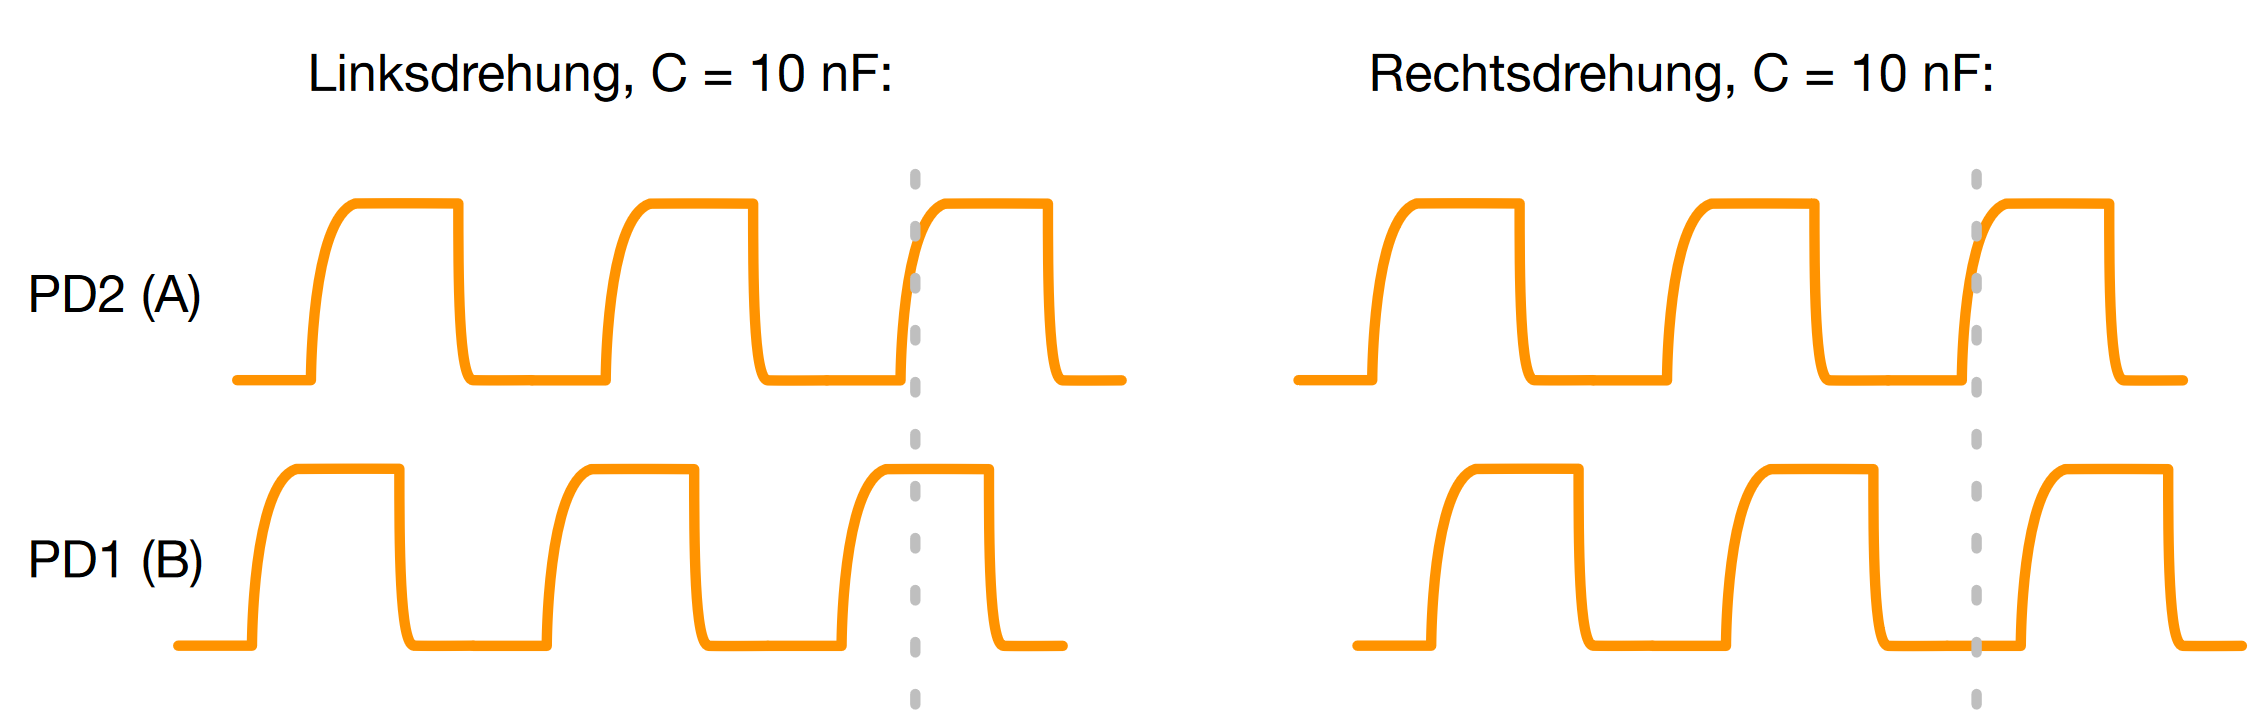
\includegraphics[width=.9\linewidth]{mikrocontroller_drehgeber.png}\\
2 Pins werden benötigt (ein Interrupt und ein normaler Eingang)\\
Pin A: Feststellen, dass gedreht wurde (Interrupt).\\
Pin B: Feststellen, in welche Richtung gedreht wurde (Eingang auslesen).\\
Zuerst wird in die ISR vom Interrupt (A) gesprungen. Dort wird dann folgendes geprüft:
\begin{itemize}
\item hat B High-Pegel? - Dann war es eine Linksdrehung
\item hat B Low-Pegel? - Dann war es eine Rechtsdrehung
\end{itemize}
\begin{minipage}{\columnwidth}
\subsubsection{Timer-Interrupts}
Der Zähler \texttt{TCNT$n$} wird mit der Frequenz $f=\frac{\text{clk}}{\text{Prescaler}}$ um 1 erhöht. \\
Überlauf-Interrupt, wenn \texttt{TCNT$n$}...
\begin{itemize}
\item von $2^8-1$ auf $2^8=256$ erhöht wird (bei $n\in \{0,2\}$)
\item von $2^{16}-1$ auf $2^{16}=65536$ erhöht wird (bei $n\in \{1,3\}$)
\end{itemize}
\end{minipage}

%Formelsammlung
\newpage
\lfoot{Nur zur persöhnlichen Verwendung!}
\cfoot{Quelle: \href{mailto:ldv@ei.tum.de}{Lehrstuhl für Datenverarbeitung (LDV)}} % Setzt die rechte Fußzeile
\rfoot{Stand: Wintersemester 23/24 \qquad \thepage/\pageref{LastPage}} % Setzt die rechte Fußzeile
\includepdf[pages=-, pagecommand={\thispagestyle{fancy}}]{./img/Formelsammlung.pdf}
%\includepdf[pages=-]{./img/Formelsammlung.pdf}

% ======================================================================
% End
% ======================================================================
\label{LastPage}
\end{document}
